\begin{auf}
    212
\end{auf}
Auf eine horizontal gelagerte Trommel (homogener Zylinder) der Masse $m=45.4kg$ ist ein Seil aufgewickelt, an dessen Ende eine Last von $m_1=10kg$ hängt (Ziehbrunnen).
\begin{enumerate}
    \item[\ref{eq:212_a}] Mit welcher Beschleunigung bewegt sich die Last aufgrund ihres Gewichts nach unten, wenn sich das Seil frei von der Trommel abwickelt? Reibung sowie Masse des Seiles werden vernachlässigt.
    \item[\ref{eq:212_b}] In welcher Zeit legt sie (beginnend aus der Ruhelage) eine Strecke von $20m$ zurück?
\end{enumerate}
\begin{figure}[h]
    \centering
    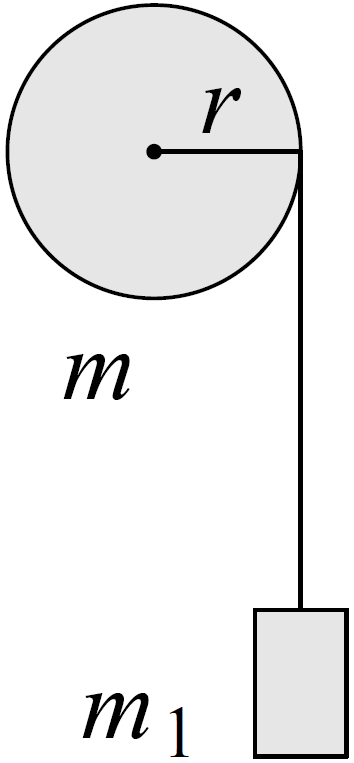
\includegraphics[height=5cm]{images/212_0.png}
    \caption{Versuchsaufbau Aufgabe 212}
\end{figure}
Die Gewichtskraft $F_G$ der Last zieht sie nach unten. Dieser wirkt die Seilkraft $F_S$ entgegen.
\begin{align}
    F&=F_G-F_S				\nonumber\\
    m_1\cdot a&=m_1\cdot g-F_S	\nonumber\\
    F_S&=m_1\cdot(g-a)	\label{eq:212_force}
\end{align}
Die Seilkraft erzeugt an der Trommel ein Drehmoment $M$.
\begin{align}
    M=F_s\cdot r	\label{eq:212_torque0}
\end{align}
Das Trägheitsmoment der Trommel $J=\frac{m\cdot r^2}{2}$, da es sich um einen Zylinder, welcher um seine Symmetrieachse rotiert. Die Winkelbeschleunigung ist ebenfalls bekannt mit $\alpha=\frac{a}{r}$.
\begin{align}
    M&=J\cdot\alpha	\nonumber\\
    M&=\frac{1}{2}\cdot m\cdot a\cdot r	\label{eq:212_torque1}
\end{align}
Man setzt \eqref{eq:212_torque0} und \eqref{eq:212_torque1} gleich. Dann setzt man \eqref{eq:212_force} ein.
\begin{align*}
    m_1\cdot(g-a)\cdot r&=\frac{1}{2}\cdot m\cdot a\cdot r\\
    m_1\cdot(g-a)&=\frac{1}{2}\cdot m\cdot a\\
    g-a&=\frac{m}{2m_1}\cdot a\\
    \frac{g}{a}-1&=\frac{m}{2m_1}\\
    \frac{g}{a}&=\frac{m+2m_1}{2m_1}\\
    a&=\frac{2m_1\cdot g}{m+2m_1}\\
    a&=\frac{2\cdot10kg\cdot9.81\frac{m}{s^2}}{45.4kg+2\cdot10kg}\\
    &\boxed{a=3\frac{m}{s^2}}	\tag{a}	\label{eq:212_a}
\end{align*}
Es handelt sich um eine gleichmäßig beschleunigte Bewegung. Das liefert den folgenden Ansatz. ($v_0=0\frac{m}{s}$, $s_0=0m$)
\begin{align*}
    s&=\frac{a}{2}t^2\\
    t^2&=\frac{2s}{a}\\
    t&=\sqrt{\frac{2s}{a}}\\
    t&=\sqrt{\frac{2\cdot20m}{3\frac{m}{s^2}}}\\
    &\boxed{t=3.65s}	\tag{b}	\label{eq:212_b}
\end{align*}